%%%%%%%%%%%%%%%%%%%%%%%%%%%%%%%%%%%%%%%%%%%%%%%%%%%%%
%%% Task 4 %%%%%%%%%%%%%%%%%%%%%%%%%%%%%%%%%%%%%%%%%%
%%%%%%%%%%%%%%%%%%%%%%%%%%%%%%%%%%%%%%%%%%%%%%%%%%%%%
\task{Single-phase active front end rectifier}
% Task "1 phasiger Wechselrichter" from ETH exam handbook (not exercise handbook) -> page 35
% Skip question 1) -> mostly PWM related, handled with another task of this exam
% Use: All subquestions of 2.) and d) from "Theoriefragen" -> fault case all transistors conduct
\taskGerman{Einphasiger aktiver Gleichrichter}

The circuit shown in \autoref{fig:Fig_Single-phase_DC_Inverter} is a single-phase DC converter.
It supplies the DC link of a locomotive, from which the traction motors are fed from the mains side. The converter uses PWM for modulation. All components are ideal, the voltage $U_\mathrm{1}$ is constant.

\begin{germanblock}
Gegegeben sei die in \autoref{fig:Fig_Single-phase_DC_Inverter} dargestellte Schaltung mit einem einphasigen Gleichspannungswechselrichter.
Er verbindet die Netzseite mit dem Gleichspannungszwischenkreis
einer Lokomotive, aus welchem die Fahrmotoren gespeist werden. Der Wechselrichter wird mit einer PWM angesteuert. Alle Bauelemente seien ideal, die Spannung $U_\mathrm{1}$ konstant.
\end{germanblock}
\input{fig/Task04/Single-phase_DC_inverter}
\begin{table}[htb]
    \caption{Parameters of the single-phase AC-DC converter.}
    \centering
    \begin{tabular}{llll}
    \toprule
    DC-link voltage: & $U_{\mathrm{1}}=\SI{1400}{\volt}$ &
    Grid voltage: & $u_{\mathrm{2i}}=\SI{1200}{\volt} \cdot \sin(\omega t)$ \\
    Grid frequency: & $f=\SI{16\frac{2}{3}}{\hertz}$ &
    Line filter: &$L=\SI{2.7}{\milli\henry}$\\
    \bottomrule
    \end{tabular}
    \label{tab:para_ACDC-conv}
\end{table}
 \subtask{Qualitatively add into \autoref{fig:subtask4.1_time} the fundamental components $u^\mathrm{(1)}_\mathrm{2}(t)$,
$u^\mathrm{(1)}_\mathrm{L}(t)$, and $i^\mathrm{(1)}_\mathrm{2}(t)$ for different operating modes of the locomotive:}{3}
\begin{itemize}
    \item starting (locomotive draws pure active power from the grid),
    \item rolling (locomotive draws neither active nor reactive power),
    \item and braking (locomotive delivers pure active power).
\end{itemize} 
\subtaskGerman{Ergänzen Sie in \autoref{fig:subtask4.1_time} qualitativ die Größen $u^\mathrm{(1)}_\mathrm{2}(t)$,
$u^\mathrm{(1)}_\mathrm{L}(t)$ sowie $i^\mathrm{(1)}_\mathrm{2}(t)$ für verschiedene Betriebsarten der Lokomotive:

\begin{itemize}
    \item Anfahren (Lok bezieht reine Wirkleistung aus dem Netz),
    \item Rollen (Lok bezieht weder Wirk- noch Blindleistung)
    \item und Bremsen (Lok gibt reine Wirkleistung ab).
\end{itemize}}
\begin{figure}[htb]
	\centering
	\begin{subfigure}[b]{0.3\textwidth}
		\centering
		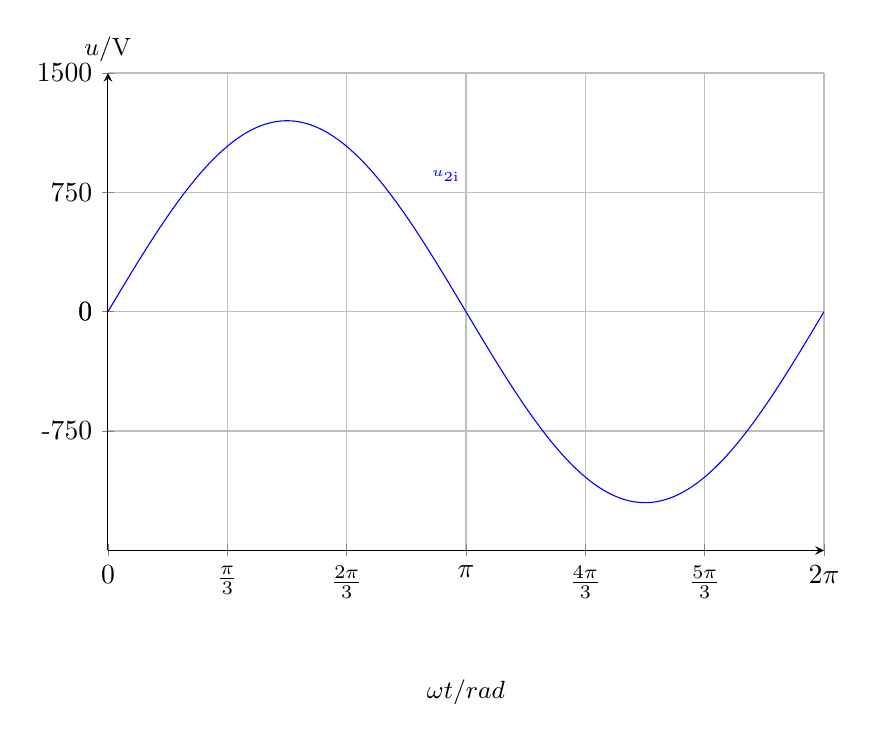
\begin{tikzpicture}
			\pgfplotsset{set layers}
			\begin{axis}[
					% x/y range adjustment
					scale only axis,
					ymin=-1500, ymax=1500,
					xmin=0, xmax=360,
					%          axis x line=none, 
					samples=500,
					axis y line=center,
					axis x line=bottom,
					extra y ticks=0,
					% Label text
					xlabel={\small$\omega t / \text{rad}$},
					ylabel={\small$u/\mathrm{V}$},
					% Label adjustment
					x label style={at={(axis description cs:0.5,-0.25)},anchor=north},
					y label style={at={(axis description cs:0,.97)},anchor=south,yshift=0.2cm},
					width=0.75\textwidth,
					height=0.5\textwidth,
					% x-Ticks
					xtick={0,60,120,180,240, 300, 360},
					xticklabels={0,$\frac{\pi}{3}$,$\frac{2\pi}{3}$,$\pi$,$\frac{4\pi}{3}$, $\frac{5\pi}{3}$, $2\pi$},
					xticklabel style = {anchor=north},
					% y-Ticks
					ytick={-1500,-750,0,750,1500},
					yticklabels={-1500,-750,0,750,1500},
					yticklabel style = {anchor=east},
					% Grid layout
					grid,
					%grid style={line width=.1pt, draw=gray!10},
					%major grid style={line width=.2pt,draw=gray!90},
				]
				% signal u_i
				\addplot[blue, domain= 0:360, solid] {1200*sin(x)};
				% Label of u_2i
				\node[blue, fill=white, inner sep = 1pt, anchor = south] at (axis cs:170,800) {\tiny$u_\mathrm{2i}$};
			\end{axis}
		\end{tikzpicture}
		\caption{Starting}
		\label{fig:time:Starting}
	\end{subfigure}
	\hfill
	\begin{subfigure}[b]{0.3\textwidth}
		\centering
		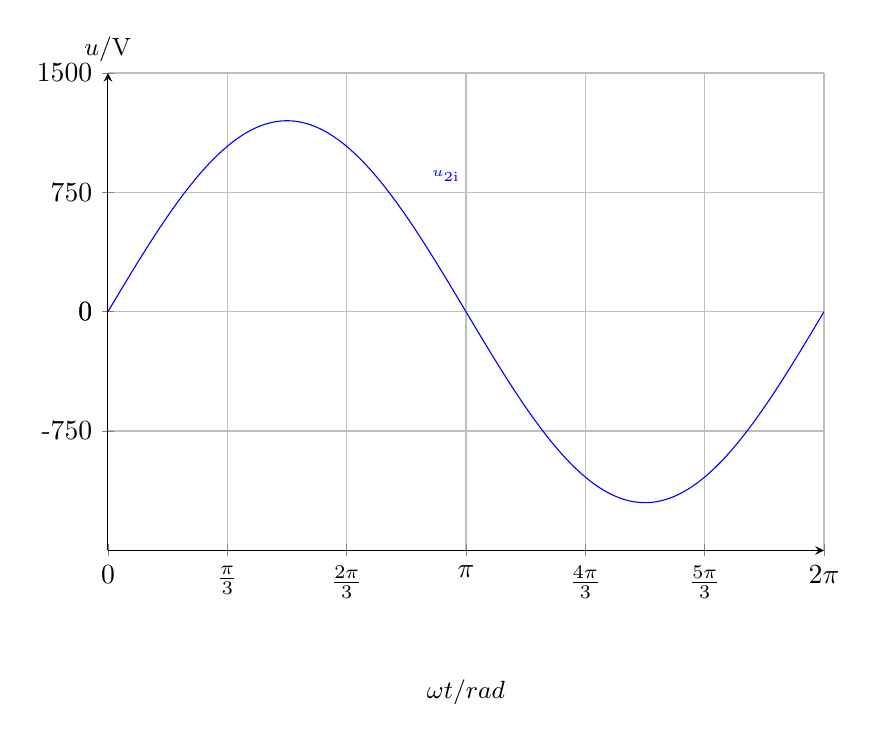
\begin{tikzpicture}
			\pgfplotsset{set layers}
			\begin{axis}[
					% x/y range adjustment
					scale only axis,
					ymin=-1500, ymax=1500,
					xmin=0, xmax=360,
					%          axis x line=none, 
					samples=500,
					axis y line=center,
					axis x line=bottom,
					extra y ticks=0,
					% Label text
					xlabel={\small$\omega t / \text{rad}$},
					ylabel={\small$u/\mathrm{V}$},
					% Label adjustment
					x label style={at={(axis description cs:0.5,-0.25)},anchor=north},
					y label style={at={(axis description cs:0,.97)},anchor=south,yshift=0.2cm},
					width=0.75\textwidth,
					height=0.5\textwidth,
					% x-Ticks
					xtick={0,60,120,180,240, 300, 360},
					xticklabels={0,$\frac{\pi}{3}$,$\frac{2\pi}{3}$,$\pi$,$\frac{4\pi}{3}$, $\frac{5\pi}{3}$, $2\pi$},
					xticklabel style = {anchor=north},
					% y-Ticks
					ytick={-1500,-750,0,750,1500},
					yticklabels={-1500,-750,0,750,1500},
					yticklabel style = {anchor=east},
					% Grid layout
					grid,
					%grid style={line width=.1pt, draw=gray!10},
					%major grid style={line width=.2pt,draw=gray!90},
				]
				% signal u_i
				\addplot[blue, domain= 0:360, solid] {1200*sin(x)};
				% Label of u_2i
				\node[blue, fill=white, inner sep = 1pt, anchor = south] at (axis cs:170,800) {\tiny$u_\mathrm{2i}$};
			\end{axis}
		\end{tikzpicture}
		\caption{Rolling}
		\label{fig:time:Rolling}
	\end{subfigure}
	\hfill
	\begin{subfigure}[b]{0.3\textwidth}
		\centering
		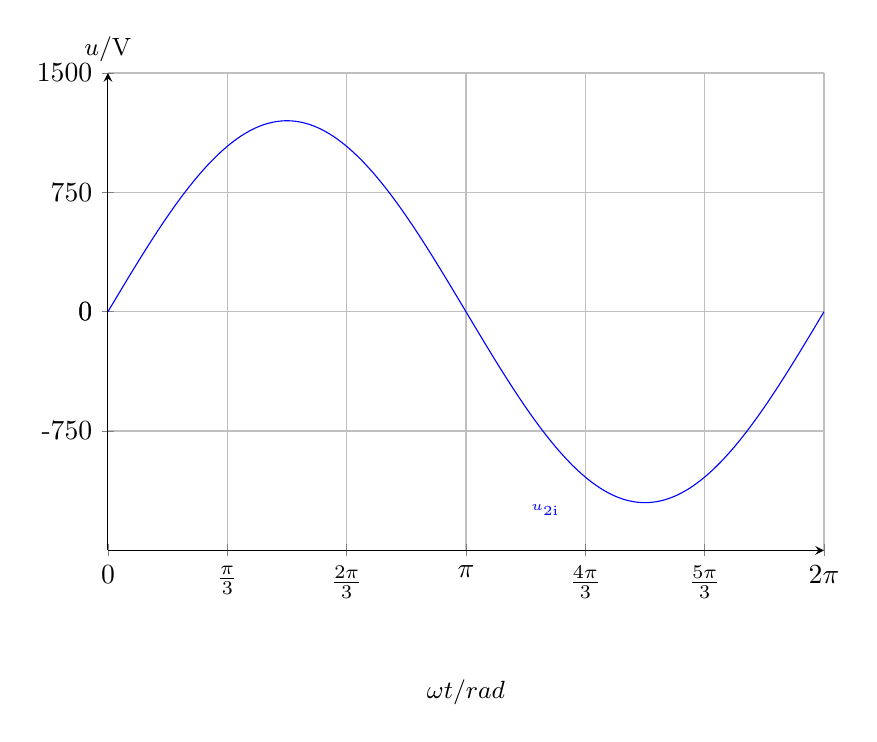
\begin{tikzpicture}
			\pgfplotsset{set layers}
			\begin{axis}[
					% x/y range adjustment
					scale only axis,
					ymin=-1500, ymax=1500,
					xmin=0, xmax=360,
					%       axis x line=none, 
					samples=500,
					axis y line=center,
					axis x line=bottom,
					extra y ticks=0,
					% Label text
					xlabel={\small$\omega t / \text{rad}$},
					ylabel={\small$u/\mathrm{V}$},
					% Label adjustment
					x label style={at={(axis description cs:0.5,-0.25)},anchor=north},
					y label style={at={(axis description cs:0,.97)},anchor=south,yshift=0.2cm},
					width=0.75\textwidth,
					height=0.5\textwidth,
					% x-Ticks
					xtick={0,60,120,180,240, 300, 360},
					xticklabels={0,$\frac{\pi}{3}$,$\frac{2\pi}{3}$,$\pi$,$\frac{4\pi}{3}$, $\frac{5\pi}{3}$, $2\pi$},
					xticklabel style = {anchor=north},
					% y-Ticks
					ytick={-1500,-750,0,750,1500},
					yticklabels={-1500,-750,0,750,1500},
					yticklabel style = {anchor=east},
					% Grid layout
					grid,
					%grid style={line width=.1pt, draw=gray!10},
					%major grid style={line width=.2pt,draw=gray!90},
				]
				% signal u_i
				\addplot[blue, domain= 0:360, solid] {1200*sin(x)};
				% Label of u_2i
				\node[blue, fill=white, inner sep = 1pt, anchor = south] at (axis cs:220,-1300) {\tiny$u_\mathrm{2i}$};
			\end{axis}
		\end{tikzpicture}
		\caption{Braking}
		\label{fig:time:Braking}
	\end{subfigure}
	\caption{Signals $u^\mathrm{(1)}_\mathrm{2}(t)$,
		$u^\mathrm{(1)}_\mathrm{L}(t)$, $i^\mathrm{(1)}_\mathrm{2}(t)$ in different operating modes.}
	\label{fig:subtask4.1_time}
\end{figure}
\begin{solutionblock}
%The phasor diagram \ref{fig:converter_single_phase_transistor_phasors} illustrates the relation between $u_\mathrm{2i}$, $u^\mathrm{(1)}_\mathrm{2}(t)$, $u^\mathrm{(1)}_\mathrm{L}(t)$, and $i^\mathrm{(1)}_\mathrm{2}(t)$ and the corresponding plot in the time domain is shown in Fig. \ref{fig:Parameters_plots}.
In starting case, since only active power is drawn current $i^\mathrm{(1)}_\mathrm{2}(t)$ will be in phase with $u_\mathrm{2i}$. Moreover, as inductors oppose changes in current (Lenz's law), the voltage across the inductor leads the current by $\SI{\frac{\pi}{2}}{\radian}$. Applying KVL at the inductor side leads to:
$$ u^\mathrm{(1)}_\mathrm{2} = u^\mathrm{(1)}_\mathrm{L} +  u_\mathrm{2i}.$$
Consequently, the resulting $u^\mathrm{(1)}_\mathrm{2}(t)$ will be leading $u_\mathrm{2i}$ by angle $0 < \varphi_2 < \SI{\frac{\pi}{2}}{\radian}$, as shown in Fig. \ref{sfig:phasor:Starting}.\\

During rolling neither active nor reactive power is drawn by the locomotive. As a result, no current flows through the inductor $i^\mathrm{(1)}_\mathrm{2}(t) = 0$. From the inductor current-voltage equation
$$ u^\mathrm{(1)}_\mathrm{L} = L \frac{\mathrm{d}i^\mathrm{(1)}_\mathrm{2}(t)}{\mathrm{d}t},$$
we can see that the voltage $u^\mathrm{(1)}_\mathrm{L}$ will be zero as well. Observing $u^\mathrm{(1)}_\mathrm{2} = u^\mathrm{(1)}_\mathrm{L} +  u_\mathrm{2i}$, this would lead to $u^\mathrm{(1)}_\mathrm{2} = 0 +  u_\mathrm{2i} = u_\mathrm{2i}$.\\

Lastly, while braking the locomotive delivers pure active power. This means current direction is reversed, hence, shifted from $u_\mathrm{2i}$ by angle $\SI{\pi}{\radian}$. From Lenz's law, we can say that $u^\mathrm{(1)}_\mathrm{L}$ will be leading by $\SI{\frac{\pi}{2}}{\radian}$. As a result, $u^\mathrm{(1)}_\mathrm{2}(t)$ will be lagging by angle $0 < \varphi_2 < \SI{\frac{\pi}{2}}{\radian}$, see Fig. \ref{sfig:phasor:Braking}.\\

The corresponding time-domain plots are shown in Fig. \ref{sfig:subtask4.1_time}
\begin{solutionfigure}[htb]
	\centering
	\begin{subfigure}[b]{0.3\textwidth}
		\centering
		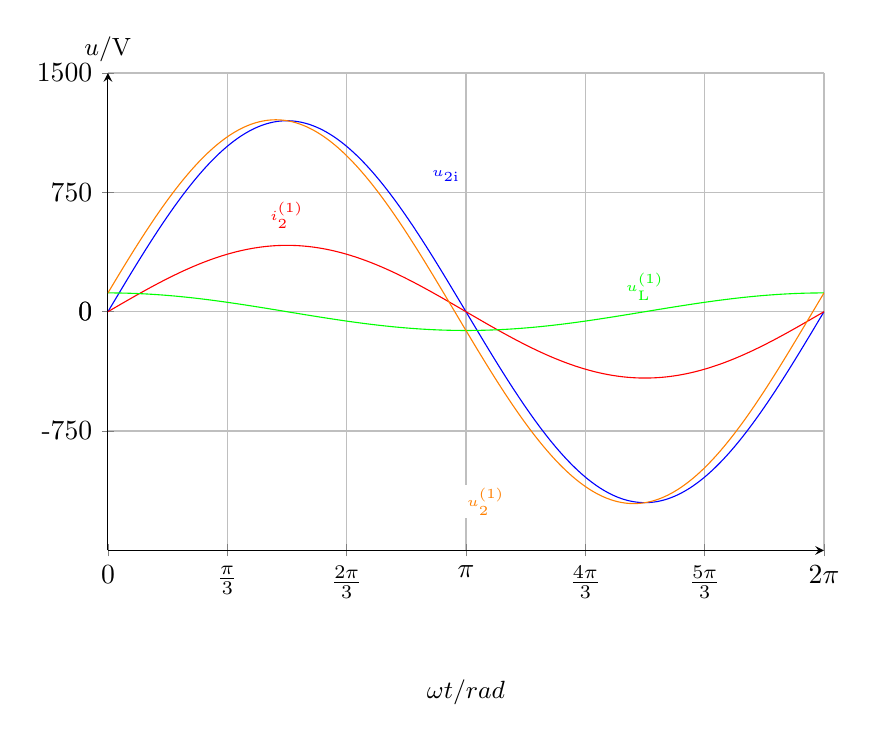
\begin{tikzpicture}
			\pgfplotsset{set layers}
			\begin{axis}[
					% x/y range adjustment
					scale only axis,
					ymin=-1500, ymax=1500,
					xmin=0, xmax=360,
					%          axis x line=none, 
					samples=500,
					axis y line=center,
					axis x line=bottom,
					extra y ticks=0,
					% Label text
					xlabel={\small$\omega t / \text{rad}$},
					ylabel={\small$u/\mathrm{V}$},
					% Label adjustment
					x label style={at={(axis description cs:0.5,-0.25)},anchor=north},
					y label style={at={(axis description cs:0,.97)},anchor=south,yshift=0.2cm},
					width=0.75\textwidth,
					height=0.5\textwidth,
					% x-Ticks
					xtick={0,60,120,180,240, 300, 360},
					xticklabels={0,$\frac{\pi}{3}$,$\frac{2\pi}{3}$,$\pi$,$\frac{4\pi}{3}$, $\frac{5\pi}{3}$, $2\pi$},
					xticklabel style = {anchor=north},
					% y-Ticks
					ytick={-1500,-750,0,750,1500},
					yticklabels={-1500,-750,0,750,1500},
					yticklabel style = {anchor=east},
					% Grid layout
					grid,
					%grid style={line width=.1pt, draw=gray!10},
					%major grid style={line width=.2pt,draw=gray!90},
				]
				% signal u_i
				\addplot[blue, domain= 0:360, solid] {1200*sin(x)};
				% Label of u_2i
				\node[blue, fill=white, inner sep = 1pt, anchor = south] at (axis cs:170,800) {\tiny$u_\mathrm{2i}$};
				% signal i^(1)_2
				\addplot[red, domain= 0:360, solid] {417*sin(x)};
				% signal u^(1)_L
				\addplot[green, domain= 0:360, solid] {118*sin(x+90)};
				% signal u^(1)_2
				\addplot[orange, domain= 0:360, solid] {1206*sin(x+5.62)};
				% Label i^(1)_2
				\node[red, fill=white, inner sep = 1pt, anchor = south] at (axis cs:90,500) {\tiny$i^\mathrm{(1)}_\mathrm{2}$};
				% Label u^(1)_L
				\node[green, fill=white, inner sep = 1pt, anchor = south] at (axis cs:270,50) {\tiny$u^\mathrm{(1)}_\mathrm{L}$};
				% Label u^(1)_2
				\node[orange, fill=white, inner sep = 1pt, anchor = south] at (axis cs:190,-1300) {\tiny$u^\mathrm{(1)}_\mathrm{2}$};
			\end{axis}
		\end{tikzpicture}
		\caption{Starting}
		\label{sfig:time:Starting}
	\end{subfigure}
	\hfill
	\begin{subfigure}[b]{0.3\textwidth}
		\centering
		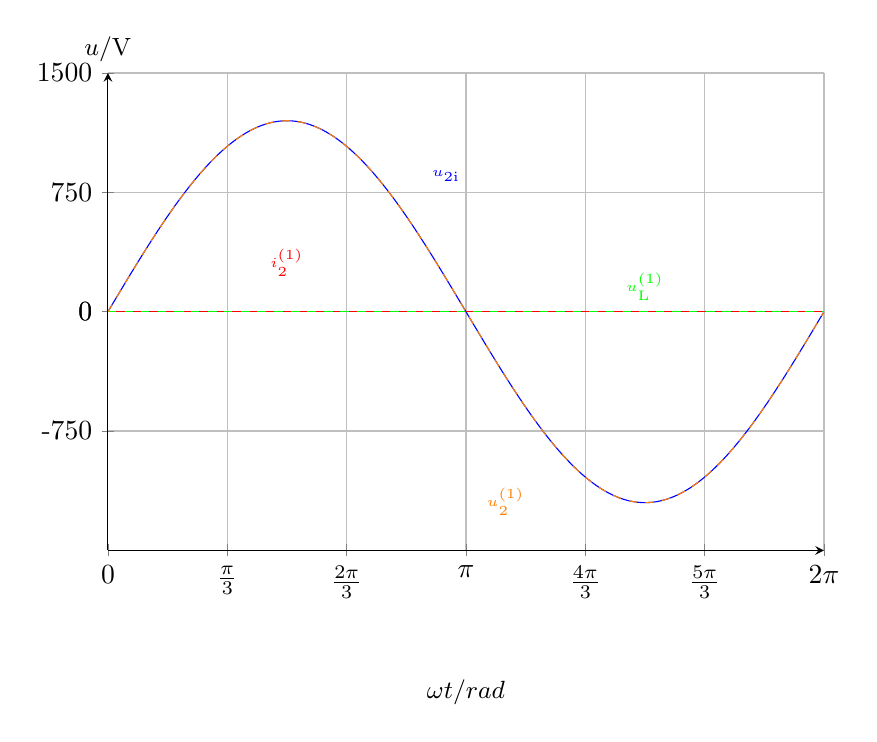
\begin{tikzpicture}
			\pgfplotsset{set layers}
			\begin{axis}[
					% x/y range adjustment
					scale only axis,
					ymin=-1500, ymax=1500,
					xmin=0, xmax=360,
					%          axis x line=none, 
					samples=500,
					axis y line=center,
					axis x line=bottom,
					extra y ticks=0,
					% Label text
					xlabel={\small$\omega t / \text{rad}$},
					ylabel={\small$u/\mathrm{V}$},
					% Label adjustment
					x label style={at={(axis description cs:0.5,-0.25)},anchor=north},
					y label style={at={(axis description cs:0,.97)},anchor=south,yshift=0.2cm},
					width=0.75\textwidth,
					height=0.5\textwidth,
					% x-Ticks
					xtick={0,60,120,180,240, 300, 360},
					xticklabels={0,$\frac{\pi}{3}$,$\frac{2\pi}{3}$,$\pi$,$\frac{4\pi}{3}$, $\frac{5\pi}{3}$, $2\pi$},
					xticklabel style = {anchor=north},
					% y-Ticks
					ytick={-1500,-750,0,750,1500},
					yticklabels={-1500,-750,0,750,1500},
					yticklabel style = {anchor=east},
					% Grid layout
					grid,
					%grid style={line width=.1pt, draw=gray!10},
					%major grid style={line width=.2pt,draw=gray!90},
				]
				% signal u_i
				\addplot[blue, domain= 0:360, solid] {1200*sin(x)};
				% Label of u_2i
				\node[blue, fill=white, inner sep = 1pt, anchor = south] at (axis cs:170,800) {\tiny$u_\mathrm{2i}$};
				% signal i^(1)_2
				\addplot[red, domain= 0:360, solid] {0*sin(x)};
				% signal u^(1)_L
				\addplot[green, domain= 0:360, dashed] {0*sin(x+90)};
				% signal u^(1)_2
				\addplot[orange, domain= 0:360, dashed] {1200*sin(x)};
				% Label i^(1)_2
				% Label i^(1)_2
				\node[red, fill=white, inner sep = 1pt, anchor = south] at (axis cs:90,200) {\tiny$i^\mathrm{(1)}_\mathrm{2}$};
				% Label u^(1)_L
				\node[green, fill=white, inner sep = 1pt, anchor = south] at (axis cs:270,50) {\tiny$u^\mathrm{(1)}_\mathrm{L}$};
				% Label u^(1)_2
				\node[orange, fill=white, inner sep = 1pt, anchor = south] at (axis cs:200,-1300) {\tiny$u^\mathrm{(1)}_\mathrm{2}$};

			\end{axis}
		\end{tikzpicture}
		\caption{Rolling}
		\label{sfig:time:Rolling}
	\end{subfigure}
	\hfill
	\begin{subfigure}[b]{0.3\textwidth}
		\centering
		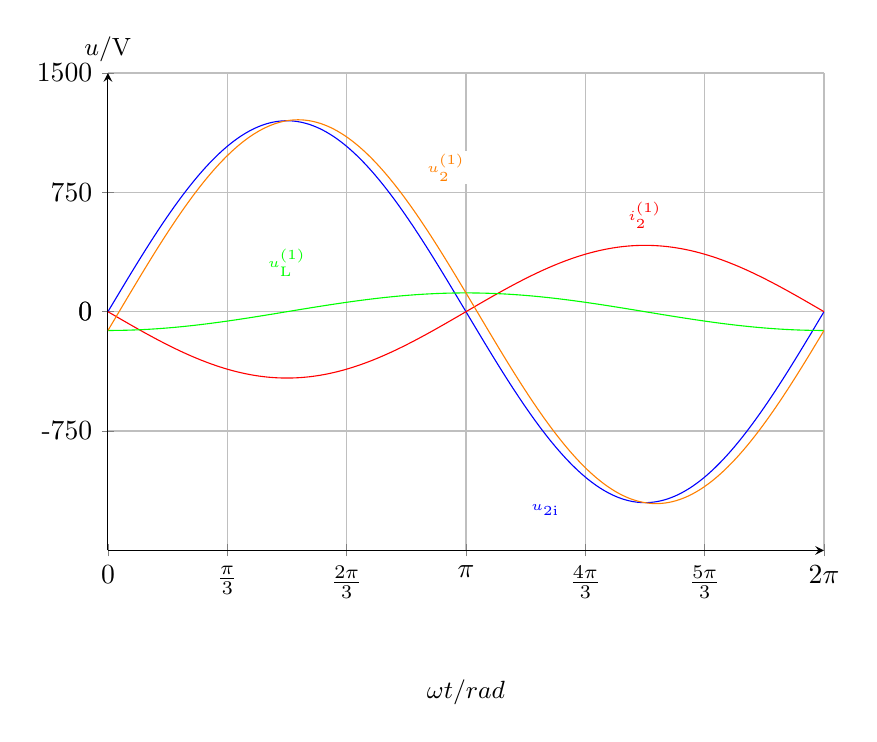
\begin{tikzpicture}
			\pgfplotsset{set layers}
			\begin{axis}[
					% x/y range adjustment
					scale only axis,
					ymin=-1500, ymax=1500,
					xmin=0, xmax=360,
					%       axis x line=none, 
					samples=500,
					axis y line=center,
					axis x line=bottom,
					extra y ticks=0,
					% Label text
					xlabel={\small$\omega t / \text{rad}$},
					ylabel={\small$u/\mathrm{V}$},
					% Label adjustment
					x label style={at={(axis description cs:0.5,-0.25)},anchor=north},
					y label style={at={(axis description cs:0,.97)},anchor=south,yshift=0.2cm},
					width=0.75\textwidth,
					height=0.5\textwidth,
					% x-Ticks
					xtick={0,60,120,180,240, 300, 360},
					xticklabels={0,$\frac{\pi}{3}$,$\frac{2\pi}{3}$,$\pi$,$\frac{4\pi}{3}$, $\frac{5\pi}{3}$, $2\pi$},
					xticklabel style = {anchor=north},
					% y-Ticks
					ytick={-1500,-750,0,750,1500},
					yticklabels={-1500,-750,0,750,1500},
					yticklabel style = {anchor=east},
					% Grid layout
					grid,
					%grid style={line width=.1pt, draw=gray!10},
					%major grid style={line width=.2pt,draw=gray!90},
				]
				% signal u_i
				\addplot[blue, domain= 0:360, solid] {1200*sin(x)};
				% Label of u_2i
				\node[blue, fill=white, inner sep = 1pt, anchor = south] at (axis cs:220,-1300) {\tiny$u_\mathrm{2i}$};

				% signal i^(1)_2
				\addplot[red, domain= 0:360, solid] {-417*sin(x)};
				% signal u^(1)_L
				\addplot[green, domain= 0:360, solid] {-118*sin(x+90)};
				% signal u^(1)_2
				\addplot[orange, domain= 0:360, solid] {1206*sin(x-5.62)};
				% Label i^(1)_2
				\node[red, fill=white, inner sep = 1pt, anchor = south] at (axis cs:270,500) {\tiny$i^\mathrm{(1)}_\mathrm{2}$};
				% Label u^(1)_L
				\node[green, fill=white, inner sep = 1pt, anchor = south] at (axis cs:90,200) {\tiny$u^\mathrm{(1)}_\mathrm{L}$};
				% Label u^(1)_2
				\node[orange, fill=white, inner sep = 1pt, anchor = south] at (axis cs:170,800) {\tiny$u^\mathrm{(1)}_\mathrm{2}$};

			\end{axis}
		\end{tikzpicture}
		\caption{Braking}
		\label{sfig:time:Braking}
	\end{subfigure}
	\caption{Signals $u^\mathrm{(1)}_\mathrm{2}(t)$,
		$u^\mathrm{(1)}_\mathrm{L}(t)$, $i^\mathrm{(1)}_\mathrm{2}(t)$ in different operating modes.}
	\label{sfig:subtask4.1_time}
\end{solutionfigure}
\end{solutionblock}

\subtask{Draw the corresponding complex phasors for the same quantities in \autoref{fig:subtask4.1_phasors}.}{3}
\subtaskGerman{Ergänzen Sie die entsprechenden komplexen Zeiger für dieselben Größen in \autoref{fig:subtask4.1_phasors}.}
\begin{figure}[htb]
	\centering
	\begin{subfigure}[b]{0.25\textwidth}
		\centering
		\begin{tikzpicture}
			\draw[->] (-0.5,0) to (3,0) node[right]{$\mathrm{Re}$};
			\draw[->] (0,-2) to (0,2) node[above]{$\mathrm{Im}$};
			\draw[->, thick, signalblue] (0,0) to (2.5,0) node[below]{$\underline{\hat{u}}_{\mathrm{2i}}$} coordinate (ug);
		\end{tikzpicture}
		\caption{Starting}
		\label{fig:phasor:Starting}
	\end{subfigure}
	\hspace*{0.2em}
	\begin{subfigure}[b]{0.25\textwidth}
		\centering
		\begin{tikzpicture}
			\draw[->] (-0.5,0) to (3,0) node[right]{$\mathrm{Re}$};
			\draw[->] (0,-2) to (0,2) node[above]{$\mathrm{Im}$};
			\draw[->, thick, signalblue] (0,0) to (2.5,0) node[below]{$\underline{\hat{u}}_{\mathrm{2i}}$} coordinate (ug);
		\end{tikzpicture}
		\caption{Rolling}
		\label{fig:phasor:Rolling}
	\end{subfigure}
	\hspace*{0.2em}
	\begin{subfigure}[b]{0.25\textwidth}
		\centering
		\begin{tikzpicture}
			\draw[->] (-2,0) to (3,0) node[right]{$\mathrm{Re}$};
			\draw[->] (0,-2) to (0,2) node[above]{$\mathrm{Im}$};
			\draw[->, thick, signalblue] (0,0) to (2.5,0) node[above]{$\underline{\hat{u}}_{\mathrm{2i}}$} coordinate (ug);
		\end{tikzpicture}
		\caption{Braking}
		\label{fig:phasor:Braking}
	\end{subfigure}
	\caption{Steady-state phasor diagrams for $\underline{u}^\mathrm{(1)}_\mathrm{2}$,
		$\underline{u}^\mathrm{(1)}_\mathrm{L}$, $\underline{i}^\mathrm{(1)}_\mathrm{2}$ in different operating modes.}
	\label{fig:subtask4.1_phasors}
\end{figure}


\begin{solutionblock}
The solution is shown in \autoref{sfig:sfig:subtask4.1_phasors}.
    \begin{solutionfigure}[htb]
     \centering
     \begin{subfigure}[b]{0.25\textwidth}
        \centering
        \begin{tikzpicture}
            \draw[->] (-0.5,0) to (3,0) node[right]{$\mathrm{Re}$};
            \draw[->] (0,-2) to (0,2) node[above]{$\mathrm{Im}$};
            \draw[->, thick, signalblue] (0,0) to (2.5,0) node[below]{$\underline{\hat{u}}_{\mathrm{2i}}$} coordinate (ug);
            \draw[->, thick, signalred] (0,0) to (1.5,0) node[below]{$\underline{\hat{i}}_{\mathrm{2}}$};
            \draw[->, thick, signalblue] (ug) to node[right]{$\underline{\hat{u}}^\mathrm{(1)}_{\mathrm{L}}$}  ++(0,1.25) coordinate (ul);
            \draw[->, thick, signalblue] (0,0) to (ul);
            \draw[->] let \p1 = (ul) in (1,0) arc(0:atan(\y1/\x1):1);
            \draw node[right] at (1.1, 0.3) {$\varphi_2$};
            \draw node[right, signalblue] at (2.2, 1.7){$\underline{\hat{u}}^\mathrm{(1)}_2$};
        \end{tikzpicture}
        \caption{Starting}
        \label{sfig:phasor:Starting}
     \end{subfigure}
    \hspace*{0.2em}
     \begin{subfigure}[b]{0.25\textwidth}
           \centering
        \begin{tikzpicture}
            \draw[->] (-0.5,0) to (3,0) node[right]{$\mathrm{Re}$};
            \draw[->] (0,-2) to (0,2) node[above]{$\mathrm{Im}$};
            \draw[->, thick, signalblue] (0,0) to (2.5,0) node[below]{$\underline{\hat{u}}_{\mathrm{2i}}$} coordinate (ug);
            \draw[->, thick, signalred] (0,0) to (0,0) node[below right]{$\underline{\hat{i}}_{\mathrm{2}}$};
            \draw[->, thick, signalblue] (0,0) to node[above right]{$\underline{\hat{u}}^\mathrm{(1)}_{\mathrm{L}}$}  ++(0,0) coordinate (ul);
            \draw[->, thick, signalblue] (0,0) to (ul);
            \draw node[right, signalblue] at (2, 0.3){$\underline{\hat{u}}^\mathrm{(1)}_2$};
        \end{tikzpicture}
        \caption{Rolling}
        \label{sfig:phasor:Rolling}
     \end{subfigure}
    \hspace*{0.2em}
     \begin{subfigure}[b]{0.25\textwidth}
         \centering
             \begin{tikzpicture}
        \draw[->] (-2,0) to (3,0) node[right]{$\mathrm{Re}$};
        \draw[->] (0,-2) to (0,2) node[above]{$\mathrm{Im}$};
        \draw[->, thick, signalblue] (0,0) to (2.5,0) node[above]{$\underline{\hat{u}}_{\mathrm{2i}}$} coordinate (ug);
        \draw[->, thick, signalred] (0,0) to (-1.5,0) node[above]{$\underline{\hat{i}}_{\mathrm{2}}$};
        \draw[->, thick, signalblue] (ug) to node[right]{$\underline{\hat{u}}^\mathrm{(1)}_{\mathrm{L}}$}  ++(0,-1.25) coordinate (ul);
        \draw[->, thick, signalblue] (0,0) to (ul) node[below]{$\underline{\hat{u}}^\mathrm{(1)}_2$};
        \draw[->] let \p1 = (ul) in (1,0) arc(0:atan(\y1/\x1):1);
        \draw node[right] at (1.1, -0.4) {$\varphi_2$};
    \end{tikzpicture}
    \caption{Braking}
     \label{sfig:phasor:Braking}
     \end{subfigure}
        \caption{Steady-state phasor diagrams.}
       \label{sfig:sfig:subtask4.1_phasors}
\end{solutionfigure}

\end{solutionblock}

\subtask{How large must the amplitude of the mains fundamental current $\hat{i}^\mathrm{(1)}_\mathrm{2}$ be if pure
fundamental active power of \SI{250}{\kilo\watt} is drawn from the grid?}{2}
\subtaskGerman{Wie groß muss die Netzstromgrundschwingungsamplitude $\hat{i}^\mathrm{(1)}_\mathrm{2}$ sein, wenn reine
Grund\-schwing\-ungs\-wirk\-leis\-tung von \SI{250}{\kilo\watt} bezogen wird?}
\begin{solutionblock}
The fundamental active power can be calculated from the effective values of the mains voltage $U_\mathrm{2i}$ as well as fundamental current $I^\mathrm{(1)}_\mathrm{2}$ using:

   $$ P^\mathrm{(1)} = U_\mathrm{2i}\cdot I^\mathrm{(1)}_\mathrm{2} = \frac{\hat{u}_\mathrm{2i}\cdot \hat{i}^\mathrm{(1)}_\mathrm{2}}{2}.$$
Solving with respect to $\hat{i}^\mathrm{(1)}_\mathrm{2}$ results in:
   $$ \hat{i}^\mathrm{(1)}_\mathrm{2} = \frac{2P^\mathrm{(1)}}{\hat{u}_\mathrm{2i}} = \frac{2 \cdot \SI{250}{\kilo\watt}}{\SI{1200}{\volt}} \approx \SI{417}{\ampere}.$$
\end{solutionblock}
\subtask{How large must the fundamental amplitude $\hat{u}^\mathrm{(1)}_\mathrm{2}$ of the inverter output voltage be in the same load case of \SI{250}{\kilo\watt}?
Calculate the corresponding modulation index $m$.}{2}
\subtaskGerman{Wie groß muss die Grundschwingungsamplitude $\hat{u}^\mathrm{(1)}_\mathrm{2}$ der Wechselrichterausgangsspannung im selben Lastfall von \SI{250}{\kilo\watt} sein? Berechnen Sie den zugehörigen Modulationsindex $m$.}

\begin{solutionblock}
Recalling:
   $$ u^\mathrm{(1)}_\mathrm{2} = u^\mathrm{(1)}_\mathrm{L} +  u_\mathrm{2i}.$$
The amplitude of the inductor fundamental voltage $\hat{u}^\mathrm{(1)}_\mathrm{L}$ can be calculated from $\hat{i}^\mathrm{(1)}_\mathrm{2}$ as:

    $$\hat{u}^\mathrm{(1)}_\mathrm{L} = \hat{i}^\mathrm{(1)}_\mathrm{2} \omega L = \SI{417}{\ampere} \cdot \SI{(2 \pi 16\frac{2}{3})}{\radian/\second} \cdot \SI{2.7}{\milli \henry} \approx \SI{118}{\volt}.$$
Hence, the corresponding fundamental amplitude of the output voltage is: 

   $$ \hat{u}^\mathrm{(1)}_\mathrm{2} = \sqrt{(\hat{u}^\mathrm{(1)}_\mathrm{L})^2 + (\hat{u}_\mathrm{2i})^2} = \sqrt{(\SI{118}{\volt})^2 + (\SI{1200}{\volt}})^2 \approx \SI{1205.8}{\volt}.$$
   While the corresponding modulation index is 
    $$m = \frac{\hat{u}^\mathrm{(1)}_\mathrm{2}}{U_{\mathrm{1}}} = \frac{\SI{1205.8}{\volt}}{\SI{1400}{\volt}} \approx 0.861.$$
\end{solutionblock}
\subtask{Due to a semiconductor defect, there is a short circuit in the inverter (all transistors
conduct). What is the active and reactive power drawn from the grid in this case?}{2}
\subtaskGerman{Aufgrund eines Halbleiterdefektes gibt es einen Kurzschluss im Wechselrichter (alle Ventile
leiten). Wie groß ist in diesem Fall die aus dem Netz bezogene Wirk- und Blindleistung?}
\begin{solutionblock}
   $$ P = \SI{0}{\watt}, \quad
    Q= \frac{U_\mathrm{2i}^2}{\omega L} = \frac{(\SI{\frac{1200}{\sqrt{2}}}{\volt})^2}{\SI{(2\pi \cdot16\frac{2}{3})}{\radian/\second} \cdot \SI{2.7}{\milli \henry}} \approx \SI{2.546}{\mega \volt \ampere}.$$
\end{solutionblock}






